
\documentclass[11pt]{article}

\usepackage{graphicx}
\usepackage{epsfig}
\usepackage{caption}
\usepackage{subcaption}
\usepackage{cite}

\begin{document}

\title{Clustering Learning for Robotic Vision}
\author{Eugenio Culurciello, Jordan Bates, Jose Carrasco, Yann LeCun, Clement Farabet}
\date{\today}
\maketitle


\section{Introduction}

In the recent years the fusion of bio-inspired and neuromorphic vision models and machine learning has dominated the development of artificial vision system for the categorization of multiple objects in static frames.
Bio-inspired deep networks are computer-vision and computational-neuroscience models of the mammalian visual system implemented in deep neural networks \cite{lecun-98,hadsell-chopra-lecun-06,gregor-nips-11,Riesenhuber1999,Serre2007,Serre2010}. Most deep network architectures are composed of multiple layers (2, 3 typically), where each layer is composed of: linear two-dimensional filtering, non-linearity, pooling of data, output data normalization \cite{jarrett-iccv-09,lecun-iscas-10,boureau-icml-10}. 
Recent machine learning research has focused on the task of training such deep networks from the abundant digital data in form of image frames and videos. In particular, deep networks need to learn good feature representations for complex visual tasks such as object categorization and tracking of objects in space and time, identifying object presence and absence. These representation usually involve learning the linear filter weight values from labeled and unlabeled input data. Since labeled data is costly and often ridden with human errors \cite{Karpathy2011, Torralba2011}, the recent focus is on learning these features purely from unlabeled input data \cite{Olshausen1996, Hyvarinen2000, Hinton2006, Vincent2008, Coates2011}. These recent methods typically learn multiple layers of deep networks by training several layers of features, one layer at a time, with varying complexity of leaning models. 

Recent techniques based on unsupervised clustering algorithms are especially promising because they use simple learning methods that quickly converge \cite{Coates2011}. These algorithms are easy to setup and train and are especially suite for robotics research, because less complex knowledge of machine learning is needed, environment-specific data can be collected quickly with a few minutes of video, setup of custom size deep networks is quick and can be adapted to specific tasks. In addition, real-time operation with efficient networks can be obtained with less than a hour of training and setup, leading to direct experimentation in robotic experiments.
[[[These models are also very interesting to bio-inspired vision research because they provide a close connection between computational neuroscience and machine learning. In particular unsupervised clustering algorithms provide a simplistic model of Hebbian Learning methods, where neurons that respond to the same input are clustered.]]]

In this paper we present results obtained with unsupervised clustering algorithms on the training and operation of deep neural networks for real-time robotic vision systems. We provide simple techniques and open-source software that allows robotic researchers to use deep network in a short setup time and with little or no knowledge of machine learning necessary.
The main goal of the paper is not to present state-of-art results on a specific dataset. Rather we use standard published datasets to evaluate the performance of prototype robotic vision system for general-purpose use, where no dataset is available. It is thus not useful to train the network to perform only on one dataset, when the levels of performance would not carry over to another dataset or real-world images.
The goal is thus mainly to evaluate the use of unsupervised networks that can support at least ten frames-per-second operation on congenital hardware, such as recent laptop computers.
The paper also focuses on the advancement of deep network operation in real-time with hardware accelerators \cite{neuflow}.




\section{Methods}

In this paper we created and tested a model of unsupervised clustering algorithms that can quickly learn linear filters weight values, and also is amenable to real-time operation with conventional mobile hardware.
We used the Torch7 software for all our experiments \cite{Collobert2011}.

\subsection{Input data}
Input data was taken from the CIFAR10 \cite{Krizhevsky2009} and the Street View House Numbers (SVHN) \cite{Netzer2011} datasets. The SVHN dataset has a training size of 73,257 32x32 images and test size of 26,032 32x32 images.
the CIFAR10 dataset has training size of 20,000 32x32 images and test size of 2,000 32x32 images.

Both datasets offer a 10 categories classification task on 32 x 32 size images. The train dataset was in all cases learned to 100\% accuracy, and training was then stopped. Input data was contrast normalized separately on each RGB channel with a 9x9 gaussian filter using the Torch7 "nn.Spatial Contrastive Normalization" function.

In terms of color space, we did not convert the input images to YUV, but rather kept them in RGB to keep the model closer to biological human vision, where the retina is broadly sensitive to roughly RGB \cite{Wandell95}. Other researchers showed slight improvements using a YUV color space.


\subsection{Network architecture}
The deep neural network architecture is composed of 4 layers. Two layers of linear two-dimensional filtering and two layers of output classifier in the form of a fully connected 2-layer neural network. The first two layers were composed of a two-dimensional convolutional linear filtering stage, a L2 norm pooling stage, and a subtractive normalization layer for removing the mean of all outputs. 
The filters of the first two layers are generated with unsupervised clustering algorithms, as explained below. Training of the last two layers fully connected neural network was performed with approximately 300 epochs on the SVHN dataset on a quad-core Intel i7 laptop, or about 8 hours. Test data convergence usually only needed approximately 15 epochs.


The layers in the clustering learning network used the following sequence of operations:
\begin{enumerate}
\item SpatialSAD module: performing sum-abs-diff operation on images convolutionally with the learned CL filters
\item Spatial Subtractive Normalization: to zero the data mean
\item Tanh nonlinearity
\item L2 pooling over 2x2 regions
\item Spatial Subtractive Normalization: to zero the data mean
\end{enumerate}

In order to show the effectiveness of the learning techniques, we compared them to a standard 1-layer and a 2-layers convolutional neural network \cite{sermanet-icpr-12,boureau-icml-10,lecun-iscas-10}. The layers in the convolutional neural network used the following sequence of operations:
\begin{enumerate}
\item SpatialConvolution module
\item Tanh nonlinearity
\item L2 pooling over 2x2 regions
\item Spatial Subtractive Normalization: to zero the data mean
\end{enumerate}


All networks used 16 filters on the first layer, 128 filters on the second layer. The final classifier was always with 128 hidden units and 10 output classes for CIFAR and SVHN. Clustering learning networks used a fully connected 1st to 2nd layer, while convolutional neural networks used 1-out-of-3 and 4-out-of-16 random connection table between the input and 1st layer, and 1st and 2nd layer respectively.



\subsection{Learning}
We use k-means clustering algorithm to learn a set of 16 filters in the first layer, and 128 filters in the second layer. Both layers filters size was set to 5 x 5 pixels for the SVHN and CIFAR datasets. In CIFAR, and on the 2nd layer, we used 3 x 3 filters, as features were more spatially constrained in this dataset. Clustering used the same size patches of the normalized images, and we used 1 Million patches from each dataset to train the first layer. The second layer training was performed by passing the entire dataset through the first layer of the deep neural network. The output dataset was then used again with the same script to train another set of linear filters, by using 1 Million patches of the processed dataset.

\begin{figure}
        \centering
        \begin{subfigure}[b]{0.3\textwidth}
                \centering
                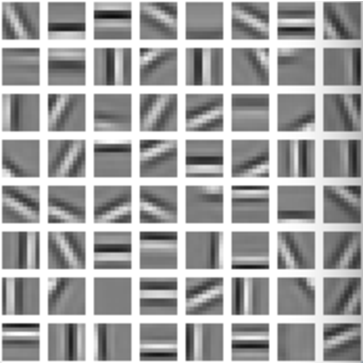
\includegraphics[width=1.2in]{filters-1l.pdf}
                \caption{1st layer filters}
                \label{fig:gull}
        \end{subfigure}%
        ~ %add desired spacing between images, e. g. ~, \quad, \qquad etc. 
          %(or a blank line to force the subfigure onto a new line)
        \begin{subfigure}[b]{0.7\textwidth}
                \centering
                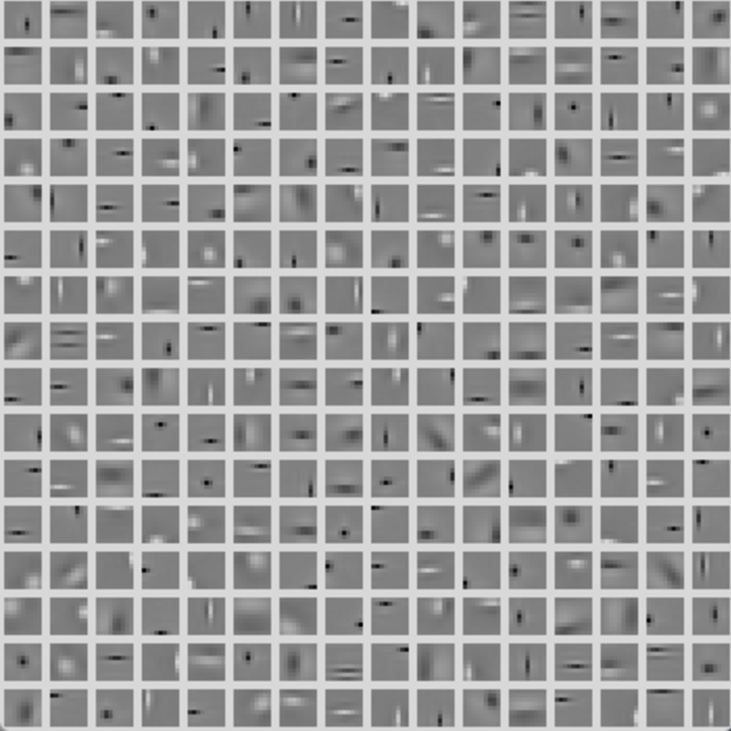
\includegraphics[width=2.4in]{filters-2l.pdf}
                \caption{2nd layer filters}
                \label{fig:tiger}
        \end{subfigure}
        \caption{Filters}\label{filters}
\end{figure}

Clustering learning filters learned on the 2nd layer used as many planes as the 1st layer (16 here). This was done to cluster different sets of features for each output of the 1st layer, and increased performance by an average of 5\% or more.


\section{Real-time network}
We use the same two-layer network architecture used in [Farabet 2012] for insuring real-time operation of ~6 frames/s on a quad-code Intel i7 laptop computer. We focused on this network and restricted ourselves to real-time operation because the goal of this project is the use of deep networks in mobile computers. The network operates on 46 x 46 input images, uses 16 7 x 7 filters on the first layer and 128 7 x 7 filters on the second layer. The network produces a 128 feature vector as output. Learned filters through clustering algorithm of size 9 x 9 were resize to size of 7 x 7 for use in this network.


TODO:  ADD TRACKING DATA FROM CL NETWORK and compare to convnet and paper \cite{Farabet 2012} 

[why 64 and 128 filters? heuristics?]


Larger network:
This network can be executed in real-time with accelerated hardware [neuflow]


Advantages:
- learning is fast: can be applied to online learning of filters, adaptation to environment?


Disadvantages:
- are clustering learning features clustered well? no copies?
- distance filtering instead of convolution?



\section{Results}

We report the results in the SVHN dataset in figure \ref{data_svhn}. Here we compared results of accuracy in the test set for 4 cases: clustering learning with 1 layer (CL 1 layer), clustering learning with 2 layers (CL 2 layers), a 1-layer and a 2-layers convolutional neural network (convnet 1l, 2l). 

\begin{figure}[htbp]
\begin{center}
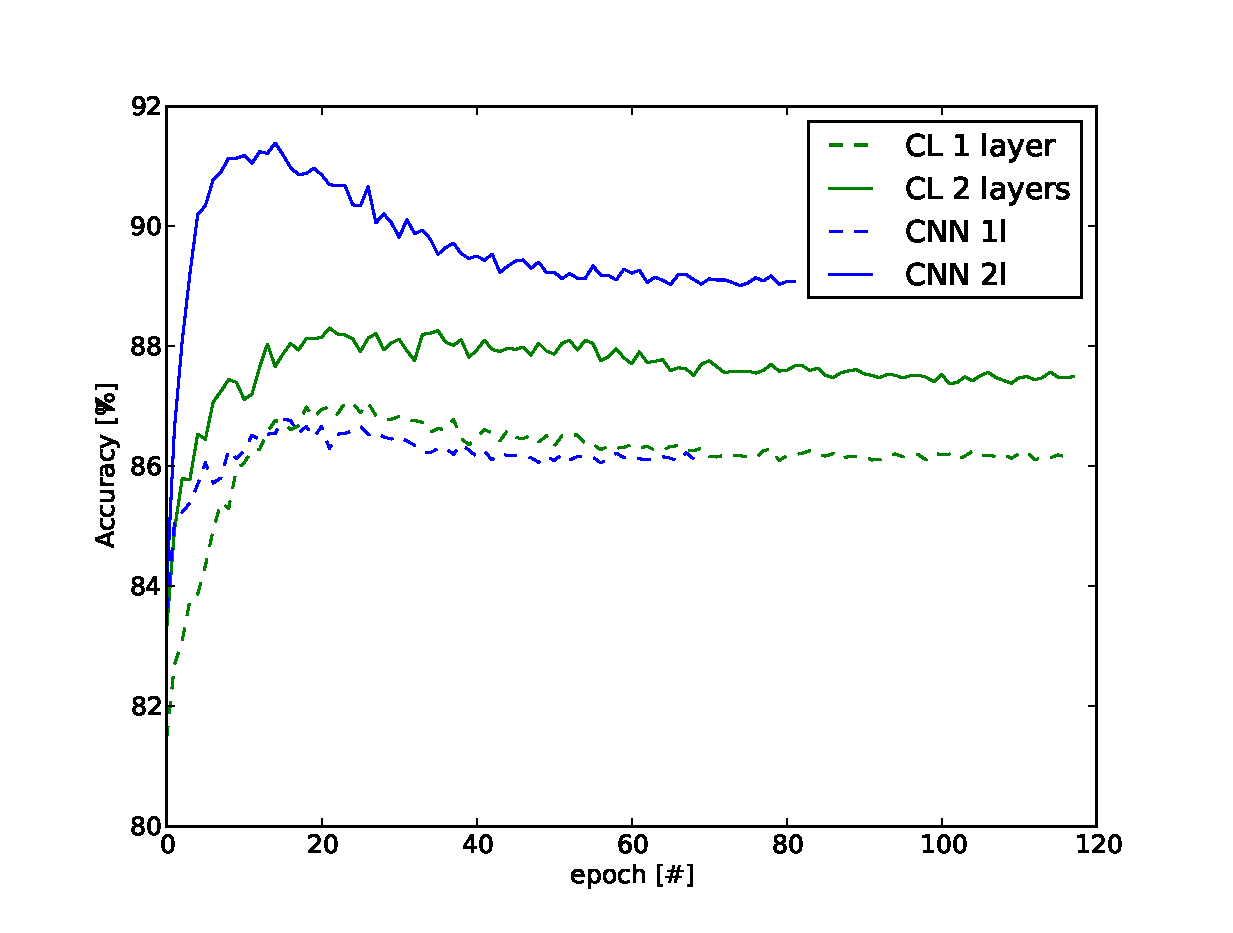
\includegraphics[width=0.8\textwidth]{data_svhn.eps}
\caption{default}
\label{data_svhn}
\end{center}
\end{figure}


The data shows that clustering learning and convnet with 1 layer provide remarkably the same levels of accuracy on the dataset. This shows that at least on the 1st layer, the features learned with clustering learning are very effective.
Adding a second layer brings the convnet to 91\% levels of accuracy, which are standard without using any sophisticated tricks and with a small network with only 16 filters on the first layer.
On the other had, the clustering learning network with 2 layers showed more than 2\% increase in accuracy, from ~86\% to ~89\%. This increase is not as large as one would want and expect from adding a second layer, but is consistent with unsupervised learning results \cite{Coates2011,Coates2011b}.

It is interesting to note that with in the clustering learning 2 layers network accuracy was above 88\%, and plateaued with the train set accuracy plateauing also at ~92\%. This shows that clustering learning filters also do not over fit, and present non-perfect, but almost identical results on both train and test sets.

The results above were all obtained with feed-forward hierarchical networks. We also tried to use multiple layers of clustering learning unsupervised networks in parallel, as recommended by other publications \cite{Coates2011,lecun-iscas-10}, but we did not obtain any benefits from that strategy, on the contrary parallel networks always reported losses of 3-5\% accuracy with respect to a single layer.


We also report here the results in the CIFAR10 dataset in figure \ref{data_cifar}. As in the SVHN case, we compared results of accuracy in the test set for 4 cases: clustering learning with 1 layer (CL 1 layer), clustering learning with 2 layers (CL 2 layers), a 1-layer and a 2-layers convolutional neural network (convnet 1l, 2l). 


\begin{figure}[htbp]
\begin{center}
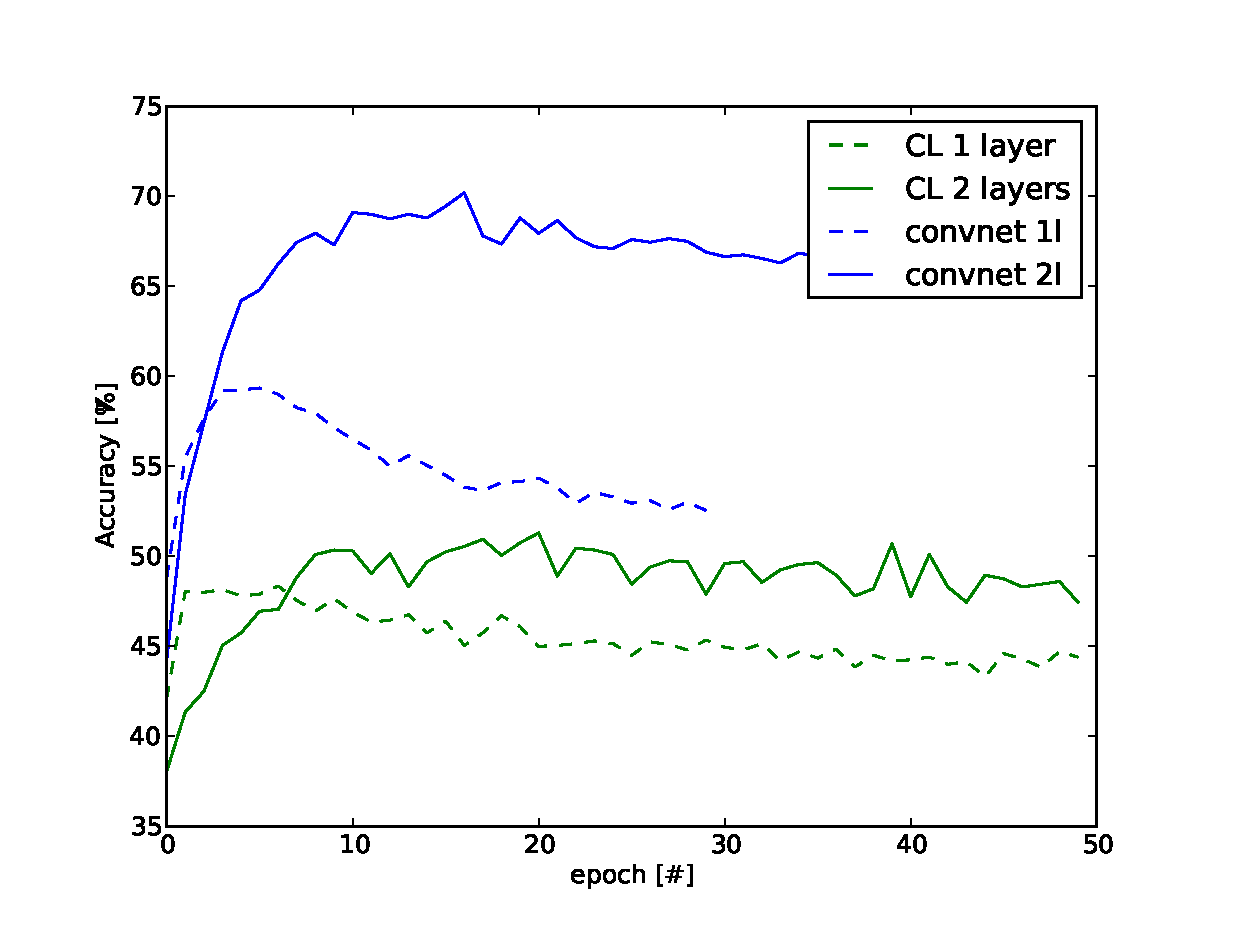
\includegraphics[width=0.8\textwidth]{data_cifar.eps}
\caption{default}
\label{data_cifar}
\end{center}
\end{figure}

The results in the CIFAR10 dataset show a gain of more than 10\% from using a single layer convnet to a 2 layer convnet. 
Clustering learning showed the same behavior as in the SVHN dataset: adding a second layer achieved 3-5\% better accuracy on the test set. This dataset uses very small images and is notoriously difficult, and clustering learning only reported a 50\% accuracy overall with 2 layers.
All results are much lower than the current state of art in this dataset, which is close to 90\%. But again we stressed our goal was real-time implementation and other researcher have obtained really hight results in this dataset only with very large networks, most of which are not amenable to real-time operation.


MORE:

x validation:
- Cifar net tested in SVHN: 1st epoch: 71% train, 76% test (almost like 1st epoch of SVHN: 74 train, 83 test - see above)
- svhn tested on CIFAr: 1st epoch: 40% train, 51% test (almost like 1st epoch of CIFAR: 37 train, 51 test - see above)

note: YUV is not bio-inspired: our photo-receptors detect intensity on broad frequencies that are similar to RGB~



\section{Discussion}

I am not sure why people would want to have popularity contests on a single dataset.�
Since I am  after general robot vision I want nets to be trained for any task.
So I did a few tests:

trained 2 nets on CIFAR10 and SVHN.
Then I tested the one from CIFAR on the SVHN dataset and vice-versa.
Results: both give chance performance.

I thought maybe this test is too rough, so I did the same, but kept the output classifier unswitched
[meaning I took the one from CIFAR and replaced the output classifier with the SVHN net, then tested on SVHN - also vice-versa]
This is equivalent to�
Results: still both perform at chance

I know these test are unfair because I did not re-train the classifier.
So I reloaded the CIFAR convnet first 2 layers and did one epoch on SVHN dataset (also vice-versa)
Results: they provide the same kind of results as the 1st epoch of the untrained network.

So I think this demonstrates my point.




Future work:
- extension to temporal filters

- Why only 2-4\% more with a second layer? and less even with a  3rd? that is a big question





Paper on Convolutional Neural Networks Applied to House Numbers Digit Classification:
\cite{sermanet-icpr-12}


\section{TODO}

- check all code for clustering learning

- get baseline performance with convnet, CIFAR, SVHN, barcelona dataset

- train with CIFAR, SVHN, barcelona Clustering learning 2 layers

- compare classification results of 1layer, 2 layers, baseline convnet

TODO: [prove that one network trained on one dataset is bad for another?]
- cross test: learn a net in barcelona, try it in another set, see performance

- test CL1l with 512, 1024, 4096 filters: replicate Adam Coates results!

- do same as above for larger filter sets with CL 2 layers!



1- continue the SpatialSAD module integration.

2 - I found out problems with learning a 2nd layer. See figure below 2nd layer filters. They are dots. It means that it is taking filters from the 1st layer and pushing them on the 2nd layer as relevant.�
Also LPP2 pooling works well, because of reasons mentioned above
We need:
- train larger set of filters on 2nd layer
- then filter out the filters that have only dot-like features, and keep the ones with more sophisticated content
we need a program to do this
- try again on SVHN or CIFAR, first using the new 2nd layer filters and seeing if we get good results.
Also feed to classifier BOTH 1st layer and 2nd layer filters, to improve recognition rate.�

3- �can you figure out how to save a net in torch without taking GB?


\begin{thebibliography} {50}

\bibitem{lecun-98} Y. LeCun, L. Bottou, Y. Bengio and P. Haffner: Gradient-Based Learning Applied to Document Recognition, Proceedings of the IEEE, 86(11):2278-2324, November 1998.

\bibitem{hadsell-chopra-lecun-06} Raia Hadsell, Sumit Chopra and Yann LeCun: Dimensionality Reduction by Learning an Invariant Mapping, Proc. Computer Vision and Pattern Recognition Conference (CVPR'06), IEEE Press, 2006.

\bibitem{gregor-nips-11} Karol Gregor, Arthur Szlam and Yann LeCun: Structured Sparse Coding via Lateral Inhibition, Advances in Neural Information Processing Systems (NIPS 2011), 24, 2011.

\bibitem{Riesenhuber1999} Riesenhuber, M. and Poggio, T. Hierarchical models of object recognition in cortex. Nature neuroscience, 2, 1999.

\bibitem{Serre2007} T. Serre, A. Oliva, T. Poggio, A feedforward architecture accounts for rapid categorization
Proceedings of the National Academy of Science, 2007.

\bibitem{Serre2010} T. Serre, T. Poggio, A neuromorphic approach to computer vision, Communications of the ACM, 2010.

\bibitem{sermanet-icpr-12}. Pierre Sermanet, Soumith Chintala and Yann LeCun: Convolutional Neural Networks Applied to House Numbers Digit Classification, Proceedings of International Conference on Pattern Recognition (ICPR'12), 2012.

\bibitem{jarrett-iccv-09} Kevin Jarrett, Koray Kavukcuoglu, Marc'Aurelio Ranzato and Yann LeCun: What is the Best Multi-Stage Architecture for Object Recognition?, Proc. International Conference on Computer Vision (ICCV'09), IEEE, 2009.

\bibitem{lecun-iscas-10} Yann LeCun, Koray Kavukvuoglu and Cl�ment Farabet: Convolutional Networks and Applications in Vision, Proc. International Symposium on Circuits and Systems (ISCAS'10), IEEE, 2010.

\bibitem{boureau-icml-10} Y-Lan Boureau, Jean Ponce and Yann LeCun: A theoretical analysis of feature pooling in vision algorithms, Proc. International Conference on Machine learning (ICML'10), 2010.

\bibitem{Coates2011} An Analysis of Single-Layer Networks in Unsupervised Feature Learning, Adam Coates, Honglak Lee, and Andrew Y. Ng. In AISTATS 14, 2011.

\bibitem{Coates2011b} A. Coates and A. Y. Ng. Selecting receptive fields in deep networks. In Advances in Neural Information Processing Systems, 2011.

\bibitem{neuflow} Eugenio Culurciello, neuFlow synthetic vision systems, http://www.neuflow.org/, 2012.

\bibitem{Olshausen1996} Olshausen, B. A. and Field, D. J. Emergence of simple- cell receptive field properties by learning a sparse code for natural images. Nature, 381(6583):607�609, 1996.

\bibitem{Hyvarinen2000} Hyvarinen, A. and Oja, E. Independent component analysis: algorithms and applications. Neural net- works, 13(4-5), 2000.

\bibitem{Hinton2006} Hinton, G., Osindero, S., and Teh, Y. A fast learning algorithm for deep belief nets. Neural Computation, 18(7), 2006.

\bibitem{Vincent2008} Vincent, P., Larochelle, H., Bengio, Y., and Manzagol, P. Extracting and composing robust features with denoising autoencoders. In International Conference on Machine Learning, 2008.

\bibitem{Karpathy2011} http://karpathy.ca/myblog/2011/04/27/lessons-learned-from-manually-classifying-cifar-10-with-code/

\bibitem{Torralba2011}
author={Torralba, A. and Efros, A.A.}, 
booktitle={Computer Vision and Pattern Recognition (CVPR), 2011 IEEE Conference on}, title={Unbiased look at dataset bias}, 
year={2011}, 
month={june}, 
volume={}, 
number={}, 
pages={1521 -1528}

\bibitem{Collobert2011} R. Collobert, K. Kavukcuoglu and C. Farabet. Torch7: A Matlab-like Environment for Machine Learning. In BigLearn, NIPS Workshop, 2011.

\bibitem{Krizhevsky2009} Learning Multiple Layers of Features from Tiny Images, http://www.cs.toronto.edu/~kriz/learning-features-2009-TR.pdf, Alex Krizhevsky, 2009.

\bibitem{Netzer2011} Yuval Netzer, Tao Wang, Adam Coates, Alessandro Bissacco, Bo Wu, Andrew Y. Ng Reading Digits in Natural Images with Unsupervised Feature Learning NIPS Workshop on Deep Learning and Unsupervised Feature Learning 2011.

\bibitem{Farabet 2012} C. Farabet, C. Couprie, L. Najman, Y. LeCun, �Scene Parsing with Multiscale Feature Learning, Purity Trees, and Optimal Covers�, in Proc. of the International Conference on Machine Learning (ICML'12), Edinburgh, Scotland, 2012.

\bibitem{Netzer2011} Yuval Netzer, Tao Wang, Adam Coates, Alessandro Bissacco, Bo Wu, Andrew Y. Ng Reading Digits in Natural Images with Unsupervised Feature Learning NIPS Workshop on Deep Learning and Unsupervised Feature Learning 2011. 

\bibitem{Wandell95} B. A. Wandell, Foundations of Vision. Sunderland, MA: Sinauer, 1995.


\end{thebibliography}



\end{document}
